\documentclass{standalone}
\usepackage{amsmath}
\usepackage{tikz}
\begin{document}
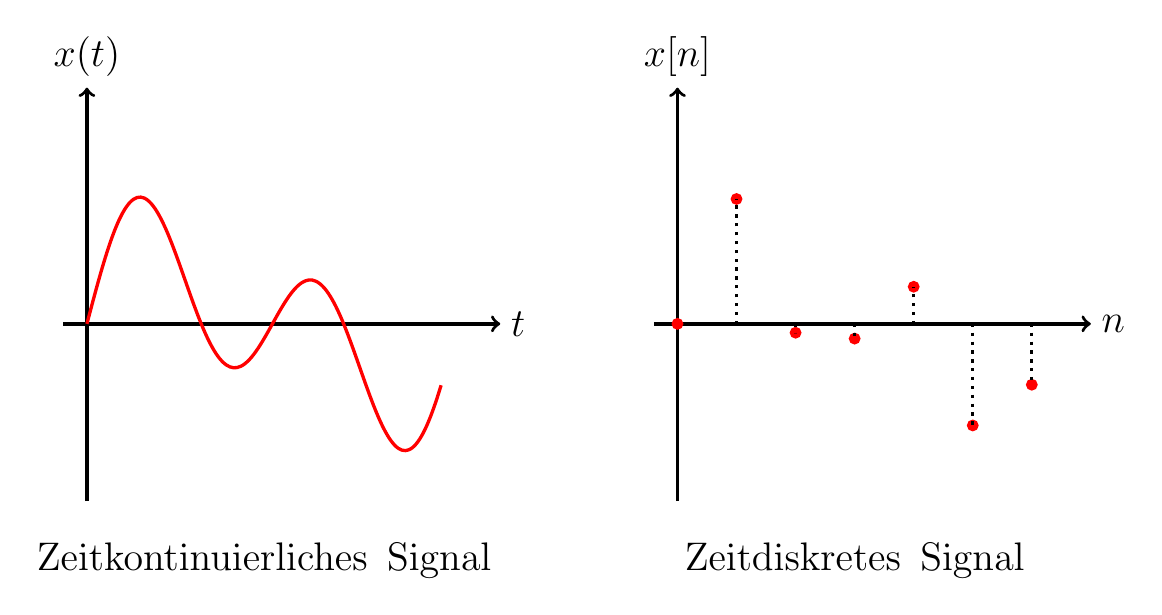
\begin{tikzpicture}[scale=1.5]

% Zeitkontinuierliches Signal (links)
\begin{scope}
    \draw[->, very thick] (-0.2,0) -- (3.5,0) node[right] {\Large $t$};
    \draw[->, very thick] (0,-1.5) -- (0,2) node[above] {\Large $x(t)$};
    
    % Das kontinuierliche Signal
    \draw[very thick, color=red,domain=0:3,samples=100,smooth] 
        plot(\x,{0.5*sin(2*\x r) + 0.7*sin(4*\x r)});
        
    \node at (1.5,-2) {\Large \text{Zeitkontinuierliches\, Signal}};
\end{scope}

% Zeitdiskretes Signal (rechts)
\begin{scope}[xshift=5cm]
    \draw[->, very thick] (-0.2,0) -- (3.5,0) node[right] {\Large $n$};
    \draw[->, very thick] (0,-1.5) -- (0,2) node[above] {\Large $x[n]$};
    
    % Das diskrete Signal (gepunktet)
    \foreach \n in {0,...,6} {
        \filldraw[red, very thick] (\n*0.5,{0.5*sin(2*\n*0.5 r) + 0.7*sin(4*\n*0.5 r)}) circle (1pt);
        \draw[dotted, very thick] (\n*0.5,0) -- (\n*0.5,{0.5*sin(2*\n*0.5 r) + 0.7*sin(4*\n*0.5 r)});
    }

    \node at (1.5,-2) {\Large \text{Zeitdiskretes\, Signal}};
\end{scope}

\end{tikzpicture}
\end{document}
